\documentclass[UTF8,ctexart,a4paper,11pt,openany]{article}
\usepackage[slantfont,boldfont]{xeCJK}
\usepackage{fontspec}
\usepackage{ctex}

\setCJKmainfont{SimSun}%[BoldFont=SimHei] %去掉注释:bf字体为黑体

\setsansfont{SimHei}
\setCJKsansfont{SimHei}

\xeCJKsetcharclass{"2160}{"2470}{1}% 1: CJK
\xeCJKsetup{AutoFallBack=true}
\setCJKfallbackfamilyfont{\CJKrmdefault}{SimSun.ttf}

%\setmainfont{Times New Roman}     %去掉注释:Times new roman字体
%\usepackage{mathptmx}             %去掉注释:Times new roman字体

\usepackage{mathtools}
\usepackage{amsmath}
\usepackage{amsfonts}
\usepackage{amssymb}
\usepackage{amsthm}
\usepackage[T1]{fontenc}
\usepackage{indentfirst} %段首空两格

\usepackage{graphicx}
\usepackage{geometry}
\usepackage{latexsym}
\usepackage{fancyhdr}
\usepackage{epstopdf}
%\usepackage{pifont}
%\usepackage[perpage,symbol*]{footmisc}
\usepackage{titlesec}
\usepackage{setspace}
\usepackage{enumerate}
\usepackage{enumitem}
\usepackage{multicol}
\usepackage{url}
\usepackage{exscale}
\usepackage{ulem}
\usepackage{relsize}
\usepackage{mathrsfs}
\usepackage{tikz}
\usepackage{wrapfig}
\usepackage{framed}
\usepackage{bm}
%\usepackage{pstricks,pst-node,multido,ifthen,calc}
\usepackage[all]{xy}
\usepackage{extarrows}
%\usepackage[backref]{hyperref}
\usepackage{hyperref}
\usepackage{stfloats} %插图的时候不分页

\setlength{\parindent}{2em} %段首空两格
\linespread{1.2}
\usepackage{listings}
\usepackage{xcolor}
\usepackage{algorithm}
\usepackage{algorithmicx}
\usepackage{algpseudocode}
\usepackage{mdframed}
\usepackage{extarrows}
\usepackage{diagbox}
\usepackage{makecell}
\usepackage{booktabs}

\theoremstyle{definition}
\mdfdefinestyle{theoremstyle}{%
linecolor=green!40,linewidth=.5pt,%
backgroundcolor=green!10,
skipabove=8pt,
skipbelow=5pt,
innerleftmargin=7pt,
innerrightmargin=7pt,
frametitlerule=true,%
frametitlerulewidth=.5pt,
frametitlebackgroundcolor=green!35,
frametitleaboveskip=0pt,
frametitlebelowskip=0pt,
innertopmargin=.4\baselineskip,
innerbottommargin=.4\baselineskip,
shadow=true,shadowsize=3pt,shadowcolor=black!20,
%theoremseparator={\hspace{1pt}},
theoremseparator={.},
nobreak=true,
}


\everymath{\displaystyle}

\newtheorem{definition}{\hspace{2em}定义}[section]
\newtheorem{axiom}{\hspace{2em}公理}

\mdtheorem[style=theoremstyle]{theorem}{定理}
\mdtheorem[style=theoremstyle]{example}{例}
\mdtheorem[style=theoremstyle]{exercise}{问题}
\newtheorem{lemma}[theorem]{\hspace{2em}引理}
\newtheorem{corollary}[theorem]{\hspace{2em}推论}

\newcommand*{\QED}{\hfill\ensuremath{\square}}
\newcommand*{\rmk}{\textbf{注:}}
\renewcommand*{\proof}{\textbf{证明:}}
\newcommand*{\tips}{\textbf{提示:}}
\newcommand*{\hard}{\textbf{\color{red}(难)}}
\newcommand*{\eqsmall}{\setlength\abovedisplayskip{1pt}\setlength\belowdisplayskip{1pt}}
\geometry{left=2cm,right=2cm,top=2cm,bottom=2cm}
% \title{数值分析上机报告(示例}
% \author{Fiddie}
\pagestyle{fancy}
\fancyfoot[C]{}
\fancyhead[RO]{ \thepage}
\fancyhead[LE]{\thepage  }
% \fancyhead[RE]{\rightmark (By Fiddie)}
% \fancyhead[LO]{\leftmark (By Fiddie)}
\titleformat{\chapter}{\centering\huge\bfseries}{第\,\thechapter\,章}{1em}{} %更改标题样式
\titleformat{\section}{\bfseries\Large}{$\S$\,\thesection\,}{1em}{} %更改标题样式
\titlespacing*{\chapter}{0pt}{9pt}{0pt} %调整标题间距
\setenumerate[1]{itemsep=0pt,partopsep=0pt,parsep=\parskip,topsep=0pt} %设置enumerate行间距
\setenumerate[2]{itemsep=0pt,partopsep=0pt,parsep=\parskip,topsep=0pt} %设置enumerate行间距
\setitemize[1]{itemsep=0pt,partopsep=0pt,parsep=\parskip,topsep=0pt} % 设置itemize行间距
\setlist[enumerate,2]{label=(\arabic*),topsep=0mm,itemsep=0mm,partopsep=0mm,parsep=\parskip}
    % 设置二层枚举为(1)样式
    
\newfontfamily\hei{SimHei}
\newcommand\textcf[1]{\textbf{\textsf{\hei{#1}}}}

\newcommand\e{\leftarrow}
%\renewcommand{\bibname}{参考文献}

\begin{document}
\begin{center}
{\huge \textbf{数值分析第8次上机作业}}

{\large 学号:221840189,姓名:王晨光}
\end{center}

\section{问题一}
    \subsection{问题}
    数学上可以证明$$\int_{0}^{1}\frac{4}{1+x^2} \mathrm{d}x = \pi .$$
    请通过数值积分来求$\pi$的近似值.
    \begin{enumerate}
        \item 分别使用复合梯形, 复合 Simpson 求积公式计算$\pi$的近似值. 选择不同的$h$, 对每种求积公式, 试将误差刻画成$h$的函数, 并比较两种方法的精度. 是否存在某个$h$, 当低于这个值之后再继续减小$h$的值, 计算不再有所改进? 为什么?
        \item 实现 Romberg 求积方法, 并重复上面的计算.
        \item 实现自适应积分方法,并重复上面的计算.
    \end{enumerate}
    \subsection{算法思路}
        \begin{itemize}
            \item \textbf{复合梯形公式: } \\ 考虑选点$$a=x_1<x_2<\cdots<x_{n+1}=b$$ 将积分区间$[a,b]$ 分为$n$个相等子区间, 且满足 $$x_{i+1}-x_i=\frac{b-a}{n}=h \Leftrightarrow x_i=a+(i-1)h$$ 在每个子区间上使用梯形公式可以得到$$\begin{aligned} \int_{x_{i}}^{x_{i+1}} f(x) d x & =\frac{h}{2}\left[f\left(x_{i}\right)+f\left(x_{i+1}\right)\right]-\frac{h^{3}}{12} f^{\prime \prime}\left(\xi_{i}\right), \\ x_{i} & <\xi_{i}<x_{i+1} .\end{aligned}$$于是得到$$\begin{aligned} \int_{a}^{b} f(x) d x & =\sum_{i=1}^{n} \int_{x_{t}}^{x_{i+1}} f(x) d x \\ & =\frac{h}{2} \sum_{i=1}^{n}\left[f\left(x_{i}\right)+f\left(x_{i+1}\right)\right]-\frac{h^{3}}{12} \sum_{i=1}^{n} f^{\prime \prime}\left(\xi_{i}\right) .\end{aligned}$$不妨设$f^{''}$在$[a,b]$上连续, 则$\exists \xi \in (a,b)$使得$$\frac{1}{n} \sum_{i=1}^{n} f^{\prime \prime}\left(\xi_{i}\right)=f^{\prime \prime \prime}(\xi)$$从而得到$$\int_{a}^{b} f(x) d x=\frac{h}{2}\left[f(a)+f(b)+2 \sum_{i=1}^{n-1} f(a+i h)\right]-\frac{n h^{3}}{12} f^{\prime \prime}(\xi)$$最终得到复合梯形公式$$T_{n}(f)=\frac{h}{2}\left[f(a)+f(b)+2 \sum_{i=1}^{n-1} f(a+i h)\right], h=\frac{b-a}{n}$$且$$I(f)=\int_{a}^{b} f(x) d x=T_{n}(f)+E_{n}(f)$$其中$$E_{n}(f)=-\frac{n h^{3}}{12} f^{\prime \prime}(\xi)=-\frac{h^{2}(b-a)}{12} f^{\prime \prime}(\xi), a<\xi<b$$
            \item \textbf{复合 Simpson 公式: } \\ 考虑$2m+1$个选点$$a=x_0<x_1<\cdots<x_{2m}=b$$ 将积分区间$[a,b]$ 分为$m$个相等的子区间, 设$x_{2i-1}$为$x_{2i}$和$x_{2i-2}$的中点, 且满足 $$x_{2i}-x_{2i-1}=\frac{b-a}{m}=2h$$ 在每个子区间上使用Simpson公式得到$$\int_{x_{2 i-2}}^{x_{2 t}} f(x) d x=\frac{h}{3}\left[f\left(x_{2 i-2}\right)+4 f\left(x_{2 i-1}\right)+f\left(x_{2 i}\right)\right]-\frac{h^{3}}{90} f^{(4)}\left(\xi_{i}\right)$$其中$x_{2i-2}<\xi<x_{2i}$. 于是, 则有: $$\begin{aligned}
                & \int_{a}^{b} f(x) d x=\sum_{i=1}^{m} \int_{x_{2 l-2}}^{x_{2 i}} f(x) d x \\
                = & \frac{h}{3}\left[\sum_{i=1}^{m}\left(f\left(x_{2 i-2}\right)+4 f\left(x_{2 i-1}\right)+f\left(x_{2 i}\right)\right)\right]-\frac{h^{5}}{90} \sum_{i=L}^{m} f^{(4)}\left(\xi_{i}\right) \\
                = & \frac{h}{3}\left[f(a)+f(b)+4 \sum_{i=1}^{m} f(a+(2 i-1) h)+2 \sum_{i=1}^{m-1} f(a+2 i h)\right] \\
                & -\frac{m h^{5}}{90} f^{(4)}(\xi),
                \end{aligned}$$这样, 便得到复合 Simpson 公式: $$\begin{array}{c}S_{m}(f)=\frac{h}{3}\left[f(a)+f(b)+4 \sum_{i=1}^{m} f(a+(2 i-1) h)+2 \sum_{i=1}^{m-1} f(a+2 i h)\right] \\ h=\frac{b-a}{2 m}=\frac{b-a}{n}\end{array}$$ 其离散误差为: $$E_{m}(f)=-\frac{m h^{5}}{90} f^{(4)}(\xi), a<\xi<b$$    
                \begin{algorithm}[H]
                    \caption{复合 Simpson 公式计算积分}
                    \begin{algorithmic}[1] %每行显示行号
                        \Require 积分区间$[a,b]$; 正整数$m$; 积分函数$f$.
                        \Ensure $I(f)=\int_{a}^{b} f(x) \mathrm{d} x$的近似值$\widetilde{I}$
                        \Function {Simpson Integral}{$a,b,m,f(x)$}
                            \State $h \e (b-a)/2m$
                            \State $\widetilde{I}_0 \e f(a)+f(b)$, $\widetilde{I}_1 \e 0$, $\widetilde{I}_2 \e 0$
                            \For {$i=1$ to $2m-1$}
                                \State $x\e a+ih$
                                \If {$i$为偶数}
                                    \State $\widetilde{I}_2 \e \widetilde{I}_2+f(x)$
                                \Else
                                    \State $\widetilde{I}_1 \e \widetilde{I}_1+f(x)$
                                \EndIf
                            \EndFor 
                            \State $\widetilde{I} \e \frac{h}{3}\left(\widetilde{I}_0+4 \widetilde{I}_1+2 \widetilde{I}_2\right)$
                            \State \Return $\widetilde{I}$
                        \EndFunction
                    \end{algorithmic}
                \end{algorithm}
            \item \textbf{Romberg 求积方法: } \\ 引入 Euler-Maclaurin 公式: $$\begin{aligned} I(f)= & T_{n}(f)-h^{2} q_{2}(0)\left[f^{\prime}(b)-f^{\prime}(a)\right] \\ & -h^{4} q_{4}(0)\left[f^{\prime \prime \prime}(b)-f^{\prime \prime \prime}(a)\right]+\cdots \\ & +(-1)^{k-1} h^{k} q_{k}(0)\left[f^{(k-1)}(b)-f^{(k-1)}(a)\right]+R_{k}^{n}(f) .\end{aligned}$$ 其中 $$R_{k}^{n}(f)=(-1)^{k} h^{k+1} \sum_{i=1}^{n} \int_{0}^{1} f^{(k)}\left(x_{i}+t h\right) q_{k}(t) d t$$我们取$k=2p$, 得到: $$I(f)-T_{n}(f)=\alpha_{2} h^{2}+\alpha_{4} h^{4}+\cdots+\alpha_{2 p} h^{2 p}+R_{2 p}^{n}(f)$$ 其中: $$\alpha_{2 j}=-q_{2 j}(0)\left[f^{(2 j-1)}(b)-f^{(2 j-1)}(a)\right], \quad 1 \leq j \leq p$$ 则有: $$I(f)-T_{n}(f)=\alpha_{2} h^{2}+\alpha_{4} h^{4}+O\left(h^{6}\right)$$ 将积分区间$[a, b]$分成$2^{m-1}$等分, 得到:$$\begin{array}{c}I(f)-T_{m, 1}=\alpha_{2} h_{m}^{2}+ \alpha_{4} h_{m}^{4}+ O\left(h_{m}^{6}\right), \\ h_{m}=\frac{b-a}{2^{m-1}} .\end{array}$$ 将积分区间$[a, b]$分成$2^{m-2}$等分, 得到:$$I(f)-T_{m-1,1}=2^{2} \alpha_{2} h_{m}^{2}+2^{4} \alpha_{4} h_{m}^{4}+O\left(h_{m}^{6}\right)$$ 整理得到: $$I(f)-\frac{1}{3}\left(4 T_{m, 1}-T_{m-1,1}\right)=\alpha_{4}^{\prime} h^{4}+O\left(h^{6}\right), \alpha_{4}^{\prime}=-4 \alpha_{4}$$ 记$T_{m, 2}=\frac{4 T_{m, 1}-T_{m-1,1}}{3}, \quad m \geq 2$ 它的离散误差是$O(h^4)$. 事实上, $T_{m,2}$恰是把积分区间$[a, b]$分成$2^{m-2}$等分的复合 Simpson 公式, 即$$T_{m,2}=S_{2^{m-2}}(f), m\geqslant 2$$进一步整理, 可以得到$$T_{m, j}=\frac{4^{j-1} T_{m, j-1}-T_{m-1, j-1}}{4^{j-1}-1}, \quad j=2,3, \cdots ; m=2,3, \cdots$$综上所述, Romberg 积分法的计算公式为: $$\begin{aligned} & T_{1,1}=\frac{h_{1}}{2}(f(a)+f(b)), \quad h_{1}=b-a, \\ T_{i, 1}= & \frac{1}{2}\left[T_{i-1,1}+h_{i-1} \sum_{k=1}^{2^{i-1}} f\left(a+\left(k-\frac{1}{2}\right) h_{i-1}\right)\right], \quad i=2,3, \cdots,\end{aligned}$$ 其中$$h_{i}=\frac{b-a}{2^{i-1}}=\frac{1}{2} h_{i-1}$$ 以及$$T_{m, j}=\frac{4^{j-1} T_{m, j-1}-T_{m-1, j-1}}{4^{j-1}-1}, \quad j=2,3, \cdots ;(m \geq j)$$实际计算$T_{m,j}$的简化如下:     
            \begin{algorithm}[H]
                \caption{Romberg 积分法}
                \begin{algorithmic}[1]
                    \Require 积分区间$[a,b]$; 正整数$m$; 积分函数$f$.
                    \Ensure Romberg积分矩阵$T$
                    \Function {Romberg Integral}{$a,b,m,f(x)$}
                        \State $h\e b-a$, $T_{1,1}\e h(f(a)+f(b))/2$
                        \For {$i=2,\cdots,m$}
                            \State $T_{2,1}\e \frac{1}{2}[T_{1,1}+h\sum_{k=1}^{2^{i-2}}f(a+(k-0.5))h]$
                            \For {$j=2,\cdots,i$}
                                \State $T \e \frac{4^{j-1}T_{2,j-1}-T_{1,j-1}}{4^{j-1}-1}$
                            \EndFor
                            \State $h\e h/2$
                            \For {$j=1,\cdots,i$}
                                \State $T_{1,j}\e T_{2,j}$
                            \EndFor
                        \EndFor
                        \State \Return $T$
                    \EndFunction
                \end{algorithmic}
            \end{algorithm}
            \item \textbf{自适应积分方法:} \\ 考虑自适应积分法与复合梯形公式积分的结合, 与 Simpson 积分方法的结合同理. 在计算梯形值序列的过程中, 每当算出一个梯形值$T_{m,1}$时, 判断它是否满足精确度要求的准则如下: $$\text{设}d=\left\{\begin{array}{ll}T_{m, 1}-T_{m-1,1}, & \left|T_{m, 1}\right|<K C \\ \frac{T_{m, 1}-T_{m-1,1}}{T_{m, 1}}, & \left|T_{m, 1}\right| \geq K C\end{array}\right.$$其中$KC$为误差控制常数. 实际计算时, 给定一个正整数$m_0$, 只有当$m>m_0$时采用$|d|<\varepsilon$, 否则可能出现假收敛. 
        \end{itemize}

        \par 对于问题一, 直接将积分区间代入后, 选取合适的超参数进行积分即可. 

    \subsection{结果分析}%重点(误差图、结果图、分析算法的收敛性(速度)、内存使用(时间、空间)、计算量、稳定性
    \begin{table}[H]
        \centering
        \begin{tabular}{ll}
            \toprule
            积分方法             & 结果值                \\ \midrule
            复合梯形公式           & 3.1411759869541287 \\
            复合 Simpson 公式    & 3.141592652969785  \\
            Romberg 求积方法     & 3.1415926535897225 \\
            自适应积分方法(Simpson) & 3.1415926538112613  \\ 
            真实值$\pi$ & 3.141592653589793  \\ \bottomrule
        \end{tabular}               
        \caption{问题一积分结果值}
    \end{table}
    其中复合梯形公式与复合 Simpson 公式选取的步长$h=0.05$, Romberg 求积方法的 Richardson 外推表的阶数为7阶, 自适应积分方法选取的容许误差为$10^{-7}$. \\
    观察得到对于四种积分方法, 从精确度的角度来看, Romberg 求积方法优于自适应积分方法(Simpson)优于复合 Simpson 公式优于复合梯形公式.  
    \begin{figure}[H]
        \centering
        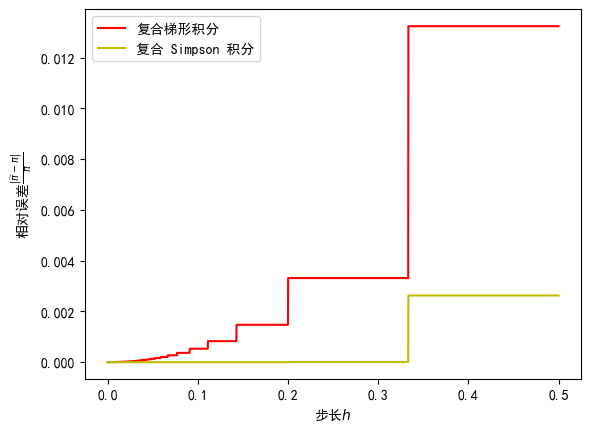
\includegraphics[width=0.6\linewidth]{pics/P8.1.png}
        \caption{相对误差随积分步长变化图}
    \end{figure}
    我们使用积分结果与$\pi$的相对误差来衡量积分方法的计算精度, 由图可以看出, 复合 Simpson 公式比复合梯形公式积分精度显著更高.
    \begin{figure}[H]
        \centering
        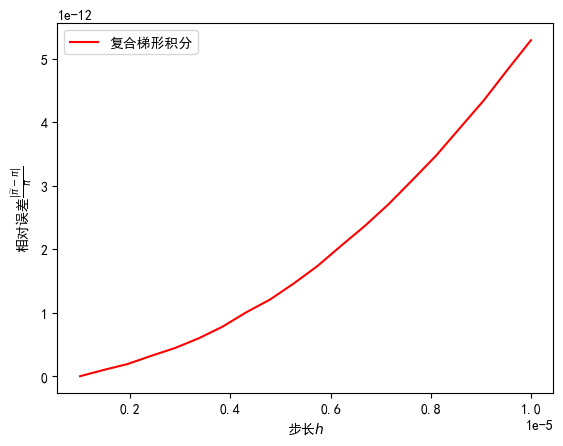
\includegraphics[width=0.6\linewidth]{pics/P8.2.png}
        \caption{相对误差随极小积分步长变化}
    \end{figure}
    由图可以看出, 即使积分步长达到$10^{-6}$量级, 积分精度还是会随$h$的减小而增大, 说明不存在这样的$h$值, 因为计算的对象函数没有线性部分, 利用线性化图形进行逼近必然存在误差, 故必然有$h$越小, 误差越小的事实. 
\section{问题二} 
    \subsection{问题}
    Planck 关于黑体辐射的理论推出积分$$\int_{0}^{\infty}\frac{x^3}{e^x - 1} \mathrm{d}x .$$
    用所掌握的所有数值积分方法计算这个积分, 并比较不同方法的计算效率和精度.
    \subsection{算法思路}
    积分方法与问题一完全一致, 但积分区间为$0$到$\infty$, 这在进行直接积分时会遇到两个问题: 
    \begin{itemize}
        \item $x=0$时函数$\frac{x^3}{e^x - 1}$无意义
        \item $x$较大时$e^x$上溢严重
    \end{itemize}
    故在考虑算法的实际实现时, 对$x<10^{-10}$全部赋值为$10^{-10}$; 对大于上溢值的$e^x$, 直接令$\frac{x^3}{e^x - 1}=0$.
    \subsection{结果分析}
    \begin{table}[H]
        \centering
        \begin{tabular}{ll}
            \toprule
            积分方法             & 结果值               \\ \midrule
            复合梯形公式           & 6.493939396095043 \\
            复合 Simpson 公式    & 6.493939412970223 \\
            Romberg 求积方法     & 6.493934406808086 \\
            自适应积分方法(Simpson) & 6.493939449769743 \\ \bottomrule
        \end{tabular}
        \caption{问题二积分结果值}
    \end{table}
    实验得到积分区间为$[30, 100]$时, 积分的结果为$10^{-11}$量级, 故最终结果为在$[0, 30]$区间内的积分值. 其中复合梯形公式与复合 Simpson 公式选取的步长$h=0.03$, Romberg 求积方法的 Richardson 外推表的阶数为7阶, 自适应积分方法选取的容许误差为$10^{-7}$. \par 由问题一的结果分析, 可以得到在计算精度上, Romberg 求积方法优于自适应积分方法(Simpson)优于复合 Simpson 公式优于复合梯形公式. \par 由问题一对于四种算法的分析过程, 可以看出Romberg 求积方法的计算效率最低; 自适应积分方法(Simpson)的计算量大于复合 Simpson 公式; 复合 Simpson 公式的计算量要大于复合梯形公式. 因此我们可以发现, 对于这四种常见积分方法, 计算精度与计算效率的比较恰好为相反关系. 
\section{结论}
    在计算精度上, Romberg 求积方法优于自适应积分方法(Simpson)优于复合 Simpson 公式优于复合梯形公式. \par
    在计算效率上, 复合梯形公式优于复合 Simpson 公式优于自适应积分方法(Simpson)优于Romberg 求积方法.
\clearpage

\section{附录: 题目一程序代码}
\lstset{
    numbers=left,
    language=Python,
    keywordstyle=\color{blue!100},
    commentstyle=\color{green!50!blue!50!},
    frame=shadowbox,%阴影
    escapeinside='',%英文分号输入中文
    xleftmargin=2em,xrightmargin=2em,aboveskip=1em,
    framexleftmargin=2em,
    extendedchars=false}

\begin{lstlisting}[aboveskip=0pt]
    import numpy as np
    def composite_trapezoidal_rule(f, a, b, n):
        h = (b - a) / n
        integral = 0.5 * (f(a) + f(b))
        for i in range(1, n):
            integral += f(a + i * h)
        integral *= h
        return integral
    
    # 定义被积函数
    def integrand(x):
        return 4 / (1 + x**2)
    
    # 设置积分区间和初始分割数
    a = 0
    b = 1
    n = 20
    
    # 使用复合梯形公式计算积分
    approx_pi_trapezoidal = composite_trapezoidal_rule(integrand, a, b, n)
    print("Approximation of pi using composite trapezoidal rule:", approx_pi_trapezoidal)
    
    def composite_simpsons_rule(f, a, b, n):
        if n % 2 != 0:
            raise ValueError("n must be even for composite Simpson's rule")
        h = (b - a) / n
        integral = f(a) + f(b)
        for i in range(1, n, 2):
            integral += 4 * f(a + i * h)
        for i in range(2, n-1, 2):
            integral += 2 * f(a + i * h)
        integral *= h / 3
        return integral
    
    # 使用复合Simpson公式计算积分
    approx_pi_simpson = composite_simpsons_rule(integrand, a, b, n)
    print("Approximation of pi using composite Simpson's rule:", approx_pi_simpson)
    
    integral1=[]
    integral2=[]
    H=np.linspace(1e-4, 0.5, 5000)
    for h in H:
        n=int(1/h)
        if n%2!=0:
            n+=1
        integral1.append(np.abs(composite_trapezoidal_rule(integrand, a, b, n)-np.pi)/np.pi)
        integral2.append(np.abs(composite_simpsons_rule(integrand, a, b, n)-np.pi)/np.pi)
    
    import matplotlib.pyplot as plt
    plt.rcParams['font.sans-serif'] = ['SimHei']  # 指定默认字体
    plt.rcParams['axes.unicode_minus'] = False
    plt.plot(H, integral1, label='复合梯形积分',  color='r')
    plt.plot(H, integral2, label='复合 Simpson 积分', color='y') 
    plt.ylabel(r'相对误差$\frac{|\widetilde{\pi}-\pi|}{\pi}$')
    plt.xlabel(r'步长$h$')
    plt.legend()
    plt.show()
    def romberg_integration(f, a, b, n):
        r = np.zeros((n, n))
        h = b - a
        r[0, 0] = 0.5 * h * (f(a) + f(b))
        for i in range(1, n):
            h /= 2
            summ = 0
            for k in range(1, 2**i, 2):
                summ += f(a + k * h)
            r[i, 0] = 0.5 * r[i-1, 0] + summ * h
            for j in range(1, i+1):
                r[i, j] = r[i, j-1] + (r[i, j-1] - r[i-1, j-1]) / ((4**j) - 1)
        return r[n-1, n-1]
    
    # 使用 Romberg 求积方法计算积分
    n_romberg = 7  # Richardson 外推表的阶数
    approx_pi_romberg = romberg_integration(integrand, a, b, n_romberg)
    print("Approximation of pi using Romberg integration:", approx_pi_romberg)
    
    def adaptive_simpson_integration(func, a, b, tol):
        # 使用Simpson积分法进行自适应积分
        h = b - a
        c = (a + b) / 2
        fa = func(a)
        fb = func(b)
        fc = func(c)
        d = (a + c) / 2
        e = (c + b) / 2
        fd = func(d)
        fe = func(e)
        S1 = h * (fa + 4 * fc + fb) / 6
        S2 = h * (fa + 4 * fd + 2 * fc + 4 * fe + fb) / 12
        if abs(S2 - S1) <= 15 * tol:
            return S2 + (S2 - S1) / 15
        else:
            left_int = adaptive_simpson_integration(func, a, c, tol / 2)
            right_int = adaptive_simpson_integration(func, c, b, tol / 2)
            return left_int + right_int
    
    # 使用自适应积分方法计算积分
    tolerance = 1e-7
    approx_pi_adaptive = adaptive_simpson_integration(integrand, a, b, tolerance)
    print("Approximation of pi using adaptive integration:", approx_pi_adaptive)
\end{lstlisting}

\clearpage



\section{附录: 题目二程序代码}
\lstset{
    numbers=left,
    language=Python,
    keywordstyle=\color{blue!100},
    commentstyle=\color{green!50!blue!50!},
    frame=shadowbox,%阴影
    escapeinside='',%英文分号输入中文
    xleftmargin=2em,xrightmargin=2em,aboveskip=1em,
    framexleftmargin=2em,
    extendedchars=false}

\begin{lstlisting}[aboveskip=0pt]
    import numpy as np
    
    # 定义被积函数
    def integrand_planck(x):
            # 定义被积函数
        if abs(x) < 1e-10:
            return x**3 / (np.exp(1e-10) - 1)
        elif x > np.log(np.inf) - 1:
            return 0
        else:
            return x**3 / (np.exp(x) - 1)
    
    # 积分区间
    a_planck = 0
    b_planck = 30
    
    # 设置 Richardson 外推表的阶数
    n_romberg_planck = 7
    
    # 设置自适应积分方法的容许误差
    tolerance_planck = 1e-6
    
    # 复合梯形求积
    n_trapezoidal = 1000
    approx_integral_trapezoidal = composite_trapezoidal_rule(integrand_planck, a_planck, b_planck, n_trapezoidal)
    
    # 复合 Simpson 求积
    n_simpson = 1000
    approx_integral_simpson = composite_simpsons_rule(integrand_planck, a_planck, b_planck, n_simpson)
    
    # Romberg 求积
    approx_integral_romberg = romberg_integration(integrand_planck, a_planck, b_planck, n_romberg_planck)
    
    # 自适应积分
    approx_integral_adaptive = adaptive_simpson_integration(integrand_planck, a_planck, b_planck, tolerance_planck)
    
    print("Approximation of the integral using composite trapezoidal rule:", approx_integral_trapezoidal)
    print("Approximation of the integral using composite Simpson's rule:", approx_integral_simpson)
    print("Approximation of the integral using Romberg integration:", approx_integral_romberg)
    print("Approximation of the integral using adaptive integration:", approx_integral_adaptive)
\end{lstlisting}

\clearpage

\bibliographystyle{unsrt}
\bibliography{Reference}
\end{document}